\documentclass[12pt,a4paper]{article}
\usepackage[utf8]{inputenc}
\usepackage{graphicx}
\usepackage{hyperref}
\usepackage{titlesec}
\usepackage{setspace}
\usepackage{lipsum}


\titleformat{\section}{\Large\bfseries}{\thesection.}{1em}{}
\titleformat{\subsection}{\large\bfseries}{\thesubsection}{1em}{}
\titleformat{\subsubsection}{\normalsize\bfseries}{\thesubsubsection}{1em}{}


\setstretch{1.3}


\title{\textbf{Comparative Analysis of Developer Surveys: \\ StackOverflow 2017 vs 2024}}
\author{Saad Almalki \\ \small Independent Researcher \\ 
\href{https://saadthelegend.netlify.app}{saadthelegend.netlify.app}}
\date{}

\begin{document}

\maketitle

\section*{Introduction}
This paper presents a basic analysis and comparison between the 2017 and 2024 
Stack Overflow Developer Surveys. This includes trends in programming languages, 
job roles, and the most popular fields. The results show an increase in the usage 
of Python, the continued dominance of JavaScript, and the emergence of more 
roles in the data science field.

\section*{Goals}
\begin{itemize}
    \item Importance of Stack Overflow surveys.
    \item Why choosing 2017 and 2024 surveys for comparison?
    \item Goals: languages, tools, database systems, job roles, and more skills.
\end{itemize}

\section*{Methodology}
\subsection*{Datasets}
\begin{itemize}
    \item Stack Overflow Developer Survey 2017 (Udacity).
    \item Stack Overflow Developer Survey 2024 (Kaggle).
\end{itemize}

\subsection*{Tools}
Python, Jupyter Notebook, Pandas, Matplotlib.

\subsection*{Steps}
\begin{enumerate}
    \item Data Cleaning: handling nulls and unused fields.
    \item Basic Analysis: exploring rows and columns with Pandas.
    \item Visualization and Comparison: charts with Matplotlib.
\end{enumerate}

\section*{Results}

\subsection*{Programming Languages}
The analysis indicates significant growth in AI and data science languages 
over the last 7 years. Web development remains strong with HTML, CSS, and JavaScript.

\subsection*{Job Roles}
\begin{itemize}
    \item Growth in web jobs (back-end, front-end, full-stack) and AI.
    \item Data science and engineering jobs are stable.
    \item Decline in some roles like software and mobile developers.
\end{itemize}

\subsection*{Top 10 Famous Languages and Information}

\textbf{10. C Language} \\

\includegraphics[width=0.5\textwidth]{images/clang.jpg} \\
General-purpose language created in 1970 by Dennis Ritchie. Known as the ``mother'' of most programming languages, widely used in low-level and system programming.

\hrulefill

\textbf{9. C++} \\

\includegraphics[width=0.5\textwidth]{images/clang.jpg} \\
Extension of C with OOP features. Used in video games, ML, servers, and software engineering.

\hrulefill

\textbf{8. C\#} \\

\includegraphics[width=0.5\textwidth]{images/csharp.jpg} \\
Created by Microsoft in 2000. Popular for Windows apps, games, and back-end web.

\hrulefill

\textbf{7. Java} \\

\includegraphics[width=0.5\textwidth]{images/java.png} \\
Released in 1995 by Sun Microsystems. Still popular for Android apps, backend, and enterprise.

\hrulefill

\textbf{6. Bash / Shell} \\

\includegraphics[width=0.5\textwidth]{images/bash.png} \\
Languages used in command-line environments. Important for Git, DevOps, and security.

\hrulefill

\textbf{5. TypeScript} \\

\includegraphics[width=0.5\textwidth]{images/ts.png} \\
Introduced in 2012 by Microsoft. Enhances JavaScript and gained wide adoption in web dev.

\hrulefill

\textbf{4. Python} \\

\includegraphics[width=0.5\textwidth]{images/py.png} \\
Versatile and beginner-friendly, used in data science, AI, web dev, and more.

\hrulefill

\textbf{3. SQL} \\

\includegraphics[width=0.5\textwidth]{images/sql.png} \\
Query language for relational databases. Essential for analysis and backend systems.

\hrulefill

\textbf{2. HTML/CSS} \\

\includegraphics[width=0.5\textwidth]{images/htmlcss.png} \\
Markup and styling languages that are the foundation of the web.

\hrulefill

\textbf{1. JavaScript} \\

\includegraphics[width=0.5\textwidth]{images/js.png} \\
The language of the web. Interactive, flexible, and essential for modern applications.

\section*{Summary}
\begin{itemize}
    \item JavaScript: $\sim$36k users in 2024 vs $\sim$17k in 2017 (+110\%).
    \item HTML/CSS: 17k (2017) $\to$ 31k (2024) (+80\%). TypeScript entered top 5.
    \item Python tripled: 10k (2017) $\to$ 29k (2024) (+175\%).
    \item SQL steady: 18k $\to$ 30k (+62\%).
    \item Java stable: 17.5k $\to$ 17k.
    \item PHP dropped from top 10 by 2024.
    \item Bash/Shell rose sharply with DevOps growth.
\end{itemize}

\subsection*{Visuals}
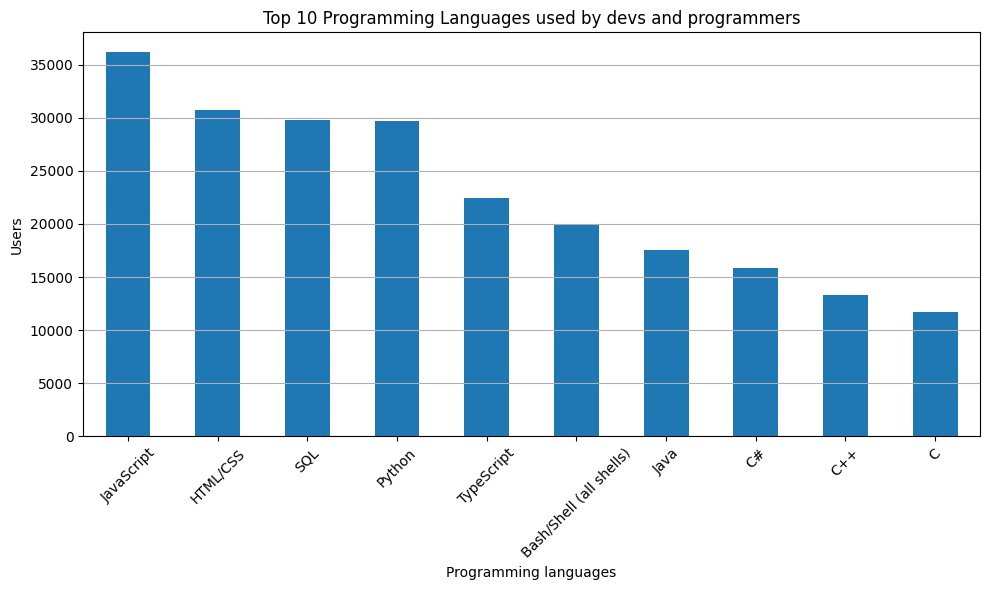
\includegraphics[width=0.8\textwidth]{images/top10-2024.jpg} \\
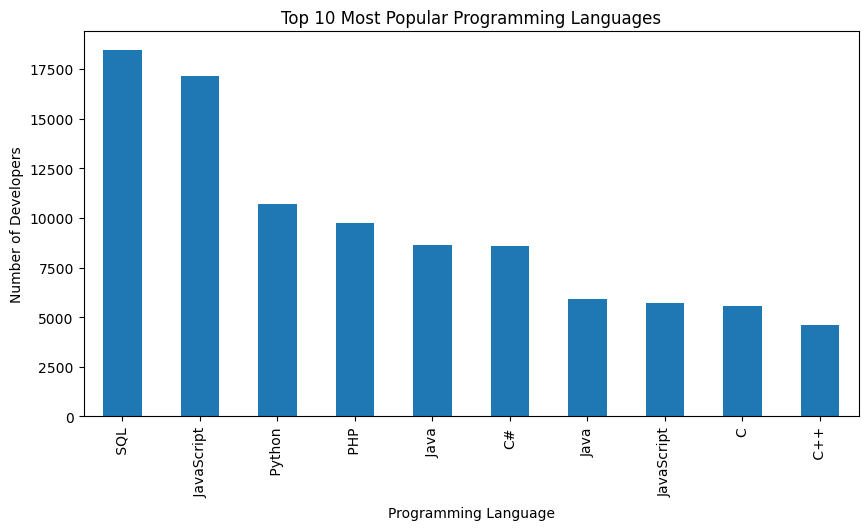
\includegraphics[width=0.8\textwidth]{images/top10-2017.png} \\
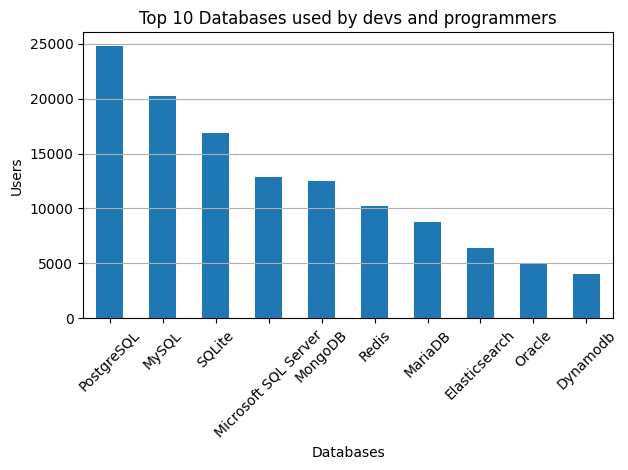
\includegraphics[width=0.8\textwidth]{images/top10-2024db.png} \\
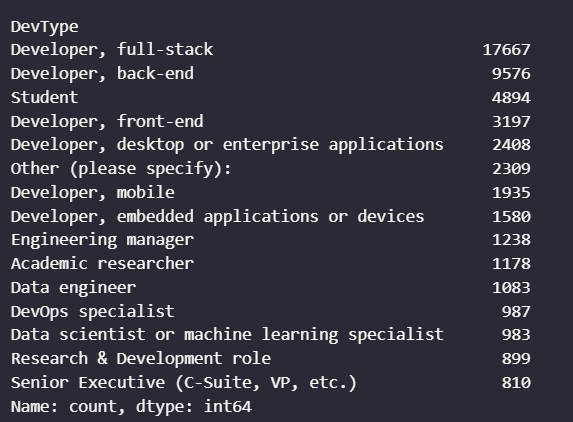
\includegraphics[width=0.8\textwidth]{images/top10-2024jobs.png} \\

\section*{Resources}
\subsection*{Source Code}
\begin{itemize}
    \item \url{https://github.com/Saad711T/Stackoverflow-2024-Survey-Analysis}
    \item \url{https://github.com/Saad711T/Udacity-IntroductionToDataScience}
\end{itemize}

\subsection*{Data}
\begin{itemize}
    \item \url{https://www.kaggle.com/datasets/berkayalan/stack-overflow-annual-developer-survey-2024}
    \item \url{https://survey.stackoverflow.co/2017}
\end{itemize}

\end{document}
